\documentclass{article}
\usepackage[utf8]{inputenc}
\usepackage{amsmath}
\usepackage{ifsym}
\usepackage{url}
\usepackage{enumitem}
\usepackage{tikz}
\usetikzlibrary{arrows}

\setlength\parindent{0pt}

\title{Query optimization homework 5}
\date{\today}

\usepackage{natbib}
\usepackage{graphicx}

\begin{document}

\maketitle

\section{Exercise 1}
\subsection{Perform the IKKBZ algorithm}

1. Call $IKKBZ(G,C_{out})$ with G: 

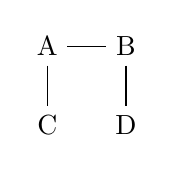
\begin{tikzpicture}
  \node (A) at (0,0) {A};
  \node (B) [right of=A] {B};
  \node (C) [below of=A] {C};
  \node (D) [right of=C] {D};
  \draw (A) -- (C);
  \draw (A) -- (B);
  \draw (B) -- (D);
\end{tikzpicture}

\newpage
2. Call $IKKBZ-Sub(G_A,C_{out})$ with $G_A:$ 

\begin{tikzpicture}
\tikzset{
    edge/.style={->,> = latex'}
}
  \node (A) at (0,0) {A};
  \node (B) at (1, -1) {B};
  \node (C) at (-1, -1) {C};
  \node (D) at (1, -2) {D};
  \draw[edge] (A) -- (C);
  \draw[edge] (A) -- (B);
  \draw[edge] (B) -- (D);
\end{tikzpicture}

\begin{table}[!hbtp]
\begin{tabular}{|l|l|l|l|l|l|}
\hline
Relation & n   & s   & C  & T  & rank           \\ \hline
B        & 10  & 0,9 & 9  & 9  & $\frac{8}{9}$  \\ \hline
C        & 100 & 0,1 & 10 & 10 & $\frac{9}{10}$ \\ \hline
D        & 100 & 0,1 & 10 & 10 & $\frac{9}{10}$ \\ \hline
\end{tabular}
\end{table}

2.1 Normalize(A) doesn't change anything\\

2.2 Merge the chains under A:

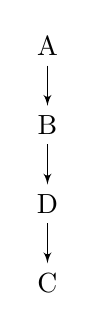
\begin{tikzpicture}
\tikzset{
    edge/.style={->,> = latex'}
}
  \node (A) at (0, 0) {A};
  \node (B) at (0, -1) {B};
  \node (C) at (0, -3) {C};
  \node (D) at (0, -2) {D};
  \draw[edge] (A) -- (B);
  \draw[edge] (B) -- (D);
  \draw[edge] (D) -- (C);
\end{tikzpicture}

\vspace*{1cm}
2.3 Denormalize$(G_A)$ doesn't change anything

2.4 Compute $C_{out}$:
\begin{align}
& C_{out}(A \bowtie B) = 10 \cdot 10 \cdot 0.9 = 90 \nonumber \\
& C_{out}((A \bowtie B) \bowtie D) = 90 \cdot 100 \cdot 0.1 + 90 = 990 \nonumber \\
& C_{out}(((A \bowtie B) \bowtie D) \bowtie C) = 900 \cdot 100 \cdot 0.1 + 990 = 9990 \nonumber
\end{align}






\newpage
3. Call $IKKBZ-Sub(G_B,C_{out})$ with $G_B:$

\begin{tikzpicture}
\tikzset{
    edge/.style={->,> = latex'}
}
  \node (A) at (-1, -1) {A};
  \node (B) at (0, 0) {B};
  \node (C) at (-1, -2) {C};
  \node (D) at (1, -1) {D};
  \draw[edge] (A) -- (C);
  \draw[edge] (B) -- (A);
  \draw[edge] (B) -- (D);
\end{tikzpicture}

\begin{table}[!hbtp]
\begin{tabular}{|l|l|l|l|l|l|}
\hline
Relation & n   & s   & C  & T  & rank           \\ \hline
A        & 10  & 0,9 & 9  & 9  & $\frac{8}{9}$  \\ \hline
C        & 100 & 0,1 & 10 & 10 & $\frac{9}{10}$ \\ \hline
D        & 100 & 0,1 & 10 & 10 & $\frac{9}{10}$ \\ \hline
\end{tabular}
\end{table}

3.1 Normalize(B) doesn't change anything\\

3.2 Merge the chains under B:

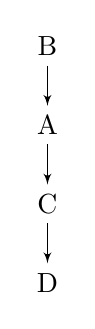
\begin{tikzpicture}
\tikzset{
    edge/.style={->,> = latex'}
}
  \node (A) at (0, -1) {A};
  \node (B) at (0, 0) {B};
  \node (C) at (0, -2) {C};
  \node (D) at (0, -3) {D};
  \draw[edge] (B) -- (A);
  \draw[edge] (A) -- (C);
  \draw[edge] (C) -- (D);
\end{tikzpicture}

\vspace*{1cm}
3.3 Denormalize$(G_B)$ doesn't change anything

3.4 Compute $C_{out}$:
\begin{align}
& C_{out}(B \bowtie A) = 10 \cdot 10 \cdot 0.9 = 90 \nonumber \\
& C_{out}((B \bowtie A) \bowtie C) = 90 \cdot 100 \cdot 0.1 + 90 = 990 \nonumber \\
& C_{out}(((B \bowtie A) \bowtie C) \bowtie D) = 900 \cdot 100 \cdot 0.1 + 990 = 9990 \nonumber
\end{align}





\newpage
4. Call $IKKBZ-Sub(G_C,C_{out})$ with $G_C:$

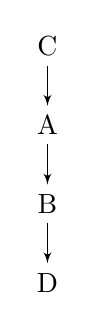
\begin{tikzpicture}
\tikzset{
    edge/.style={->,> = latex'}
}
  \node (A) at (0, -1) {A};
  \node (B) at (0, -2) {B};
  \node (C) at (0, 0) {C};
  \node (D) at (0, -3) {D};
  \draw[edge] (C) -- (A);
  \draw[edge] (A) -- (B);
  \draw[edge] (B) -- (D);
\end{tikzpicture}

\begin{table}[!hbtp]
\begin{tabular}{|l|l|l|l|l|l|}
\hline
Relation & n   & s   & C  & T  & rank           \\ \hline
A        & 10  & 0,1 & 1  & 1  & $0$  \\ \hline
B        & 10  & 0,9 & 9  & 9  & $\frac{8}{9}$  \\ \hline
D        & 100 & 0,1 & 10 & 10 & $\frac{9}{10}$ \\ \hline
\end{tabular}
\end{table}

\vspace*{1cm}
4.1 Denormalize$(G_C)$ doesn't change anything

4.2 Compute $C_{out}$:
\begin{align}
& C_{out}(C \bowtie A) = 100 \cdot 10 \cdot 0.1 = 100 \nonumber \\
& C_{out}((C \bowtie A) \bowtie B) = 100 \cdot 10 \cdot 0.9 + 100 = 1000 \nonumber \\
& C_{out}(((C \bowtie A) \bowtie B) \bowtie D) = 900 \cdot 100 \cdot 0.1 + 1000 = 10000 \nonumber
\end{align}




\newpage
5. Call $IKKBZ-Sub(G_D,C_{out})$ with $G_D:$

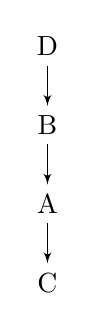
\begin{tikzpicture}
\tikzset{
    edge/.style={->,> = latex'}
}
  \node (A) at (0, -2) {A};
  \node (B) at (0, -1) {B};
  \node (C) at (0, -3) {C};
  \node (D) at (0, 0) {D};
  \draw[edge] (A) -- (C);
  \draw[edge] (B) -- (A);
  \draw[edge] (D) -- (B);
\end{tikzpicture}

\begin{table}[!hbtp]
\begin{tabular}{|l|l|l|l|l|l|}
\hline
Relation & n   & s   & C  & T  & rank           \\ \hline
A        & 10  & 0,9 & 9  & 9  & $\frac{8}{9}$  \\ \hline
B        & 10  & 0,1 & 1  & 1  & $0$  \\ \hline
C        & 100 & 0,1 & 10 & 10 & $\frac{9}{10}$ \\ \hline
\end{tabular}
\end{table}

\vspace*{1cm}
5.1 Denormalize$(G_D)$ doesn't change anything

5.2 Compute $C_{out}$:
\begin{align}
& C_{out}(D \bowtie B) = 100 \cdot 10 \cdot 0.1 = 100 \nonumber \\
& C_{out}((D \bowtie B) \bowtie A) = 100 \cdot 10 \cdot 0.9 + 100 = 1000 \nonumber \\
& C_{out}(((D \bowtie B) \bowtie A) \bowtie C) = 900 \cdot 100 \cdot 0.1 + 1000 = 10000 \nonumber
\end{align}



\newpage
6. Choose the precedence graph with the minimal cost, both $G_A$ and $G_B$ are minimal, so we choose $G_A$ and construct the following join tree:

\begin{tikzpicture}[sibling distance=1.5cm]
  \node (j1) {$\bowtie$} {
    child {
      node (j2) {$\bowtie$}
      child {
        node (j3) {$\bowtie$}
        child {
          node (j4) {$A$}
        }
        child {
          node (j5) {$B$}
        }
      }
      child {
        node (j6) {$D$}
      }
    }
    child {
      node (j7) {$C$}
    }
  };
\end{tikzpicture}

\end{document}

